\section{Introduction}

[Previous section looks at the quantity of dust across time, but this is assuming that the dust itself is the same at all epochs.]

\section{Dust Properties of DSFGs}

Interstellar dust plays a crucial role in the formation of galaxies as dust grains are the site of molecule formation like molecular hydrogen, $H_2$, the primary fuel for star formation (\citealt{Kennicutt_2012}). $H_2$ is the most abundant molecule in the Universe but is difficult to observe directly unless originating from energetic environments. Alternatives include observing less abundant molecules such as CO and using conversion factors to estimate the mass of molecular hydrogen, or observing dust emission to estimate dust masses (as in the previous chapter) and assuming gas-to-dust ratios (e.g. \citealt{Saintonge_2013}) to convert these into estimates for the total gas mass in high-redshift galaxies (e.g. \citealt{Magdis_2012}; \citealt{Eales_2012}; \citealt{Scoville_2014}; \citealt{Santini_2014}; \citealt{Genzel_2015}). Such studies have shown that galaxies at high redshift contain a higher fraction of gas than galaxies today (\citealt{Tacconi_2010}; \citealt{Scoville_2016}; \citealt{Scoville_2017}; \citealt{Millard_2020}), showing that direct observations of dust emission are useful in our understanding of how galaxies grow and evolve. It is important to note, however, that studies that make these links between dust emission and the evolution of galactic properties make the basic assumption that properties of the dust remain constant with redshift. In the following we investigate the possibility of evolution in dust itself by modelling the dust emission from a sample of high-redshift galaxies and measuring their dust properties over a large expanse of cosmic history.

Of particular importance to us is the dust emissivity spectral index, $\beta$, which controls the frequency dependence of the emissivity of dust grains per unit mass. By assuming, as is customary, that the optical depth of a galaxy can be approximated as a power law of the form $\tau \propto \nu^\beta$, we are implicity assuming that $\beta$ encodes within it information about the dust grain properties such as their chemical composition and their size and growth. The assumed value of $\beta$ for a galaxy can have significant consequences on the assumed absorption properties of the dust grains and consequently on fundamental properties of the ISM in the galaxy such as the total mass of dust (\citealt{Bianchi_2013}; \citealt{Clark_2016}).

Theoretical models for dust (e.g. \citealt{Draine_1984}; \citealt{Draine_2011}; \citealt{Kohler_2015}) predict $\beta$ values to range between approximately 1 -- 2 depending on the chemical composition of the dust grains. Adopting suitable fixed values of $\beta$ have been vital for estimates of the dust temperature and dust luminosity of galaxies in past studies, particularly for high-redshift sources that often lack constraints in the far-infrared (e.g. \todo[color=green]{Add references}). A nominal value of $\beta$ = 2 is common practice in this scenario as it mimics the emissivity of mixtures of amorphous silicates and graphites that well represent the optical properties of Galactic dust grains. However, recent studies have shown that the value of $\beta$ can take a wide variety of values among local galaxies and even among different regions within the same galaxy. For example, \citealt{Lamperti_2019} model the far-infrared dust SEDs of 192 nearby galaxies from the JCMT dust and gas In Nearby Galaxies Legacy Exploration (JINGLE) survey and observed a range of temperatures for the cold dust between 17 and 30\,K and dust emissivity spectral indices between 0.6 and 2.2. Within M31 (Andromeda) \citealt{Smith_2012}, \citealt{Draine_2014} and \citealt{Whitworth_2019} identified a decrease in $\beta$ with galactocentric radius, potentially a result of $\beta$ evolving to higher values when observed in denser regions of the ISM due to grain coagulation. A follow up study by \citealt{Athikkat-Eknath_2022} compared the average $\beta$ measured inside and outside molecular clouds within M31, and while there was no evidence to support the idea that $\beta$ varies due to dense molecular gas, the radial variation in $\beta$ remained present. At higher redshifts, where the far-infrared part of the spectrum is spatially unresolved, it is not possible to constrain the true value of a galaxy's $\beta$ but can be used to define an \textit{effective} $\beta$ value that represents the integrated dust properties over the whole galaxy. [...]\todo[color=orange]{Importance of having an effective $\beta$ value.}

\section{Obtaining Redshifts from Carbon Monoxide Lines}

In order to study the evolution of the dust properties of DSFGs we require robust redshifts to place their formation in cosmic history and to determine accurate measurements of fundamental properties. Obtaining robust ages of galaxies in the form of spectroscopically determined redshifts is hampered by the poor spatial resolution of single-dish observations, which worsens with increasing redshift. While DSFGs can be discovered at far-infrared and sub-mm wavelengths to high redshifts directly from the photometry of the sub-mm source, selecting those with distinctly red sub-mm colours in the \textit{Herschel} bands (e.g. \citealt{Dowell_2014}; \citealt{Ivison_2016}; \citealt{Donevski_2018}; \citealt{Duivenvoorden_2018}), careful consideration of the selection wavelength is required to make optimal use of the negative K-correction. For example, the \textit{Herschel}-SPIRE bands increasingly probe the peak of the dust SED at higher redshifts, making them less sensitive to unlensed DSFGs beyond z $\sim$ 2 -- 3. Additionally, the dust-obscured nature of this population of galaxies makes the identification of counterparts at other wavelengths where spectroscopically determined reshifts are readily available more difficult, which is compounded by the poor resolution and source confusion in the sub-mm (see the Likelihood Ratio analysis of Chapter \ref{chapter:Data_Release_3} for an example).

A more reliable method for robust redshifts is to follow up single-dish observations with inteferometric measurements with interferometers such as the Atacama Large Millimeter/submillimeter Array (ALMA). An even more direct way of obtaining redshfits while observing sources in the sub-mm/mm wavebands is to observe molecular emission lines which can be directly associated with the sub-mm emission without the need for intermediary steps with high-resolution imaging. Recent advancements in the possible bandwidths of instruments like ALMA and the Northern Extended Millimetre Array (NOEMA) have allowed for the ability to detect spectral lines (typically from CO or [CII]) that emanate unambiguously from the sub-mm source. CO is the second most abundant molecule in the Universe after $H_2$ and has rotational transitions that produce some of the brightest lines in the millimeter spectrum. The brightness of the CO lines result from the abundance of CO, the low excitation energy of the transitions and the wavelengths at which they occur coinciding with regions of the spectrum with high atmospheric transmission probed by ALMA. A secondary advantage of using molecular emission to determine spectroscopic redshifts is that they are independent of the photometry used to describe the dust SED and are therefore less prone to bias. In Figure \ref{fig:redshift_ladder} we show the coverage of CO line transitions as functions of the redshift and observed wavelength. We see that at [...] wavelengths, there is a non-uniform coverage of CO transitions, meaning that sources believed to be at a particular redshift may have multiple line detections, allowing for unambiguous constraints on the redshift of the galaxy, single line detections, which allows for some abiguity to the redshift solution, or no line detections. In the regions where no CO lines can be detected by a particular instrument, "redshift deserts" appear as breaks in the redshift distribution of galaxies.

\todo[color=red]{Complete figure and add caption}
\begin{figure}
	\centering
	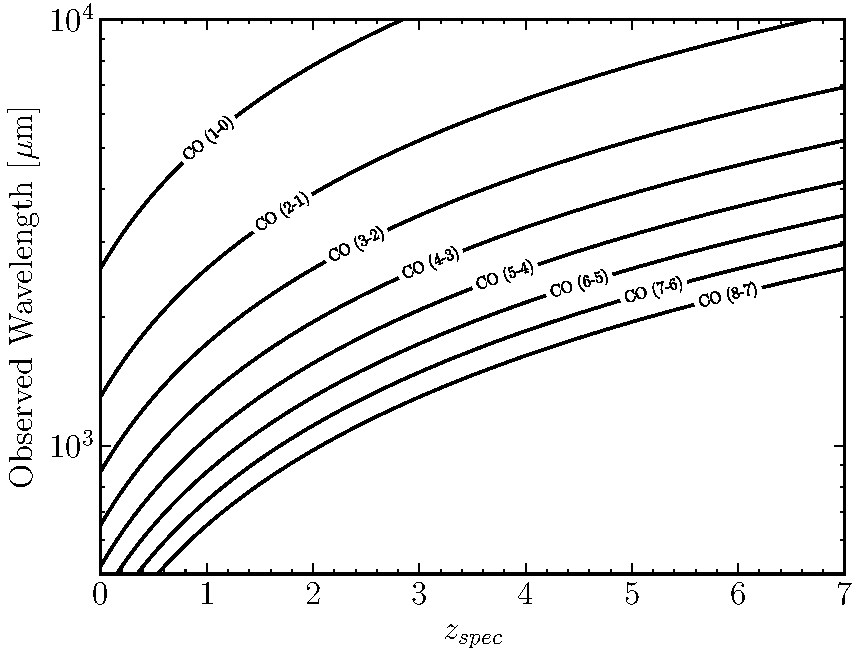
\includegraphics[width=0.5\columnwidth]{Figures/redshift_ladder.pdf}
	\caption{Caption}
	\label{fig:redshift_ladder}
\end{figure}

In this work we study bright infrared sources detected by \textit{Herschel} and the South Pole Telescope (SPT; \citealt{Carlstrom_2011}) that have spectroscopically determined redshifts to test whether their measured dust properties have evolved from the early Universe to the peak epoch of star formation (between 2 $\lesssim z_{\textrm{spec}} \lesssim$ 6). We are also interested in identifying possible diversity in the dust properties of DSFGs and whether differing selection methods influence the type of dust that is observed. We therefore implicity assume in the following work that changes in the properties of the interstellar dust in galaxies can be directly inferred from variations in the spectral index, $\beta$ and the temperature of dust grains.

\section{Sample Creation}
\subsection{South Pole Telescope DSFGs}

A population of IR-bright SMGs selected at 1.4\,mm were obtained from the South Pole Telescope - Sunyarv-Zel'dovich (SPT-SZ) survey (\citealt{Vieira_2010}; \citealt{Mocanu_2013}; \citealt{Everett_2020}) which covers approximately 2500\,deg$^2$. The depth of this survey reaches $\sim$ 20\,mJy at 1.4\,mm, corresponding to sources detected at greater than 4.5\,$\sigma$ significance. We define our SPT sample as the 81 sources that have had synchrotron dominated systems removed (based on their 1.4\,mm to 2\,mm flux density ratios) and flux-limited to $S_{\textrm{870\,\micron}}$ > 25\,mJy. The high flux density cuts imply that most IR-bright galaxies would be too faint for the SPT sample without having been magnified from gravitational lensing. As shown by \citealt{Weiss_2013}, the average magnification of these sources are $\mu \sim$ 15 (corresponding to intrinsic flux densities of $S_{1.4\,\textrm{mm}}$ = 1 -- 3\,mJy), which is similar to the flux densities of unlensed sources identified from blank field surveys in the sub-mm/mm wavebands (e.g. \citealt{Coppin_2006}; \citealt{Pope_2006}; \citealt{Weiss_2009}) and are thus likely to be representative of this population albeit at higher observed redshifts.

During ALMA Cycle 0 \citealt{Weiss_2013} conducted a blind redshift survey for 26 SPT sources with ALMA's Band 3 receiver (2.6 -- 3.6\,mm). In total 44 line features were identified in the survey as emission lines of $^{12}$CO, $^{13}$CO, CI, H$_2$O and H$_2$O$^+$. The spectra of the 26 sources could be categorized according to the ambiguity of their estimated redshifts: 12 sources had spectra with multiple clear line features, from which a unique redshift solution can be found from the ALMA scans alone; 11 had a single line feature for which other spectroscopic or photometric measurements would be requied to constrain the redshift; and three sources for which no line features were observed. The same observing strategy was used during ALMA Cycle 1 by \citealt{Strandet_2016} to extend the redshift survey of \citealt{Weiss_2013} with an additional 15 sources observed in ALMA Band 3. For sources with a single CO line detection during Cycle 0, \citealt{Strandet_2016} present ALMA 1\,mm (Band 6) follow-up observations and, when still not satisfactory, follow-up observations were made with the First Light APEX Submillimetre Heterodyne receiver (FLASH; \citealt{Heyminck_2006}), the Swedish-ESO PI receiver (SEPIA; \citealt{Billade_2012}) and the Z-spec camera (\citealt{Naylor_2003}) onboard the Atacama Pathfinder Experiment (APEX) targeting CO and [CII] lines for those that remained unambiguous during Cycles 0 and 1. Lastly, \citealt{Reuter_2020} concluded the SPT redshift survey during ALMA Cycles 3, 4 and 7 by presenting spectra for the remaining 40 of the total 81 sources that had yet to be scanned. This resulted in 41 new spectroscopic redshifts. The culmination of these studies is a sample of 81 SPT-selected DSFGs  each with a spectroscopic redshift in the range 1.9 < $z_{\textrm{spec}}$ < 6.9; the median redshift of the sample being $z_{\textrm{median}}$ = 3.9$\pm$0.2 (\citealt{Reuter_2020}).

The SPT-DSFGs have photometric coverage that fully traces the SED peak and Rayleigh-Jeans (R-J) tail of the dust emission for all sources. Most of the SPT sample have coverage that spans at least observed wavelengths between 250\,\micron and 3\,mm. This photometry includes flux densities measured at 250-, 350- and 500\,\micron (\textit{Herschel}-SPIRE), 870\,\micron (APEX-LABOCA), 1.4- and 2\,mm (SPT) and 3\,mm (ALMA). For a subset of 65 sources, 100- and 160\,\micron flux densities were measured with \textit{Herschel}-PACS. The flux densities from \textit{Herschel} were estimated by fitting a Gaussian to the SPIRE counterparts and taking the peak as the flux density at 250-, 350- and 500\,\micron, or by using apertures of 7' and 10' to extract the flux density at 100- and 160\,\micron. The LABOCA, SPT and ALMA flux densities were taken to be the peak flux density of the point sources observed on the respective continuum maps. For the 3\,mm observations with ALMA, this was estimated from the continuum maps obtained during the blind redshift search. Given the range of redshifts, the SPT sources have a minimum photometric coverage between rest frame wavelengths 83\,\micron $\lesssim \lambda_{\textrm{rest}} \lesssim$ 380\,\micron meaning that the peak of the dust emission at $\sim$ 100\,\micron is always constrained and the Rayleigh-Jeans tail is well sampled (note that in Section [...]\todo[color=green]{Add section reference when written} we place further constraints on which sources are included in this study based on the number of photometric constraints available on the R-J tail). The complete set of photometric observations for the SPT DSFGs can be found in Appendix D of \citealt{Reuter_2020} and in Appendix \ref{app:SPT_DSFG_photometry} including the estimated magnifications of each source due to gravitational lensing as measured by \citealt{Spilker_2016}. In the cases where a magnification could not be measured, the average value of $\mu$ = 5.5 is used.

\subsection{The HerBS Sample}

A second sample used in this study comes from the \textit{Herschel} Bright Sources (HerBS; \citealt{Bakx_2018}) catalogue, a sample selected from the brightest high-redshift sources detected from the H-ATLAS project. Using the SED template derived by \citealt{Pearson_2013} to represent typical H-ATLAS sources (see Section \ref{sec:phot_z_Herschel}), \citealt{Bakx_2018} estimated the redshift of each source and selected those that have a measured photometric redshift > 2 and are observed at a 500\,\micron flux density > 80\,mJy. Initially the sample consisted of 223 sources, but having removed nearby galaxies and known blazars (\citealt{Negrello_2010}; \citealt{Lopez-Caniego_2013}), the HerBS sample is reduced to 209 SMGs. Presented with the catalogue are observations at 850\,\micron with the SCUBA-2 instrument (\citealt{Holland_2013}) on the James Clerk Maxwell Telescope (JCMT) for 203 sources. A detected source with SNR$_{850\,\micron}$ > 3 and offset from the \textit{Herschel} source < 10" is observed for 159 galaxies. Given that the sensitivity of \textit{Herschel}-SPIRE observations are poor beyond redshifts z $\sim$ 2 [...]\todo[color=orange]{Give some justification here}, the selection of galaxies in the HerBS sample is limited to very bright, rare sources. A large percentage of the sample are thus lensed ultraluminous IR galaxies (ULIRGS) with far-IR luminosities in the range $10^{12} L_\odot < L_{FIR} < 10^{13} L_\odot$ and hyperluminous IR galaxies (HyLIRGS) with $L_{FIR} > 10^{13} L_\odot$.

Spectroscopic redshifts are obtained for a subset of sources in the HerBS catalogue (selected from the H-ATLAS South Galactic Pole field) as part of the Bright Extragalactic ALMA Redshift Survey (BEARS: \citealt{Urquhart_2022}; \citealt{Bendo_2023}; \citealt{Hagimoto_2023}). \citealt{Urquhart_2022} targeted 85 sources for CO line emission with ALMA and presented spectroscopic measurements for 71 sources associated with 62 HerBS fields (the ALMA Band 4 images with angular resolution of $\sim$ 2" revealed that only half of the fields contained just a single source, while several contained two or more objects with similar spectroscopic redshifts - suggesting possible locations of physially associated galaxies or single sources being lensed by a foreground deflector). The BEARS spectral line survey started in ALMA Cycles 4 and 6 using the Band 3 receiver of the Atacama Compact Array (ACA) and continued during Cycle 7 in Bands 3 and 4 with the ALMA 12\,m Array. All sources with a spectroscopic redshift have Band 3 observations with the 12\,m Array, 74 of which also have Band 3 observations. The 11 remaining sources without Band 3 observations from the 12\,m Array depend on the ACA. As shown in Figure \ref{fig:redshift_ladder} \todo[color=orange]{Check that this is illustrated} the coverage of Bands 3 and 4 allows for the detection of CO lines between (2 -- 1) and (6 -- 5) depending on the redshift of the source; \citealt{Urquhart_2022} find that line detections are primarily found from the CO(3 -- 2), (4 -- 3) and (5 -- 4) transitions (38, 36 and 28 sources respectively). The frequencies of the spectral lines are transformed to redshift solutions using the graphical method described in \citealt{Bakx_2022} and, in doing so, find redshifts for 59 sources based on multiple spectral lines suggesting an unambiguous redshift. An additional 13 sources with emission from a single line have redshift solutions that can be relied upon since the CO emission is notably bright. Since adjacent CO lines typically have similar integrated line fluxes, alternative redshift solutions can be excluded when a single strong emission line is present. HerBS sources are retained in this study if they have spectroscopic redshifts determined from a single CO line.

In the cases where the HerBS source is deblended in the ALMA images we assume that the redshift of the group is the average spectroscopic redshift of all components, providing they are within 0.1 of each other. If there is only a single redshift corresponding to one of the components (and the redshift corresponding to the integrated emission of all sources is not provided), we assume that the redshift is applicable for the whole field. While \citealt{Bendo_2023} show that the brightest component (alphanumerically labelled A for each source) produces < 80\% of the total emission at 2\,mm, it is only in 4 fields (HerBS-56, -131, -138 and -146) that the spectroscopic redshift is assumed from components that does not include the brightest.

The photometry available for HerBS sources covers a similar range to the SPT sample: \textit{Herschel}-PACS (100-, 160\,\micron), \todo[color=orange]{Include these values} \textit{Herschel}-SPIRE (250-, 350-, 500\,\micron), SCUBA-2 (850\,\micron), ALMA (2-, 3\,mm). The ALMA flux densities were serendipitously estimated from the continuum of the spectrosopic survey. We also include snapshot continuum observations in ALMA Band 6 (1.1 -- 1.4\,mm) for a selection of ultra-red objects from the H-ATLAS that were taken as part of project 2018.1.00526.S (\textit{3000 dusty starbursts at z > 4}). For sources where the reduced angular resolution of the ALMA beam resolves the HerBS source into multiple components, \citealt{Bendo_2023} report the integrated flux densities of all objects if they lie within twice the FWHM of the ALMA beam, or if they are connected by structures that are themselves detected at greater than 3$\sigma$ significance. We preferentially chose to use the integrated fluxes for each HerBS source if available, or failing this, combine fluxes of individual components providing they are all detected. For example, the HerBS-63 field showed two detected ALMA sources in the Band 4 images, while a third source appeared in the Band 3 image misaligned with the other two. The third component (HerBS-63C) may not have been detected at 2\,mm because of poor sensitivity at the edge of the 3\,mm image or because it contains some contribution from AGN emission making it much brighter at longer wavelengths. In either case this inhibits us from knowing the integrated flux in both bands for all components, assuming that they may all be physically related, and so has been left out of the sample used here. In this sense we have taken a cautious approach to combining photometry. The shorter selection wavelength compared to the SPT sample leads to a narrower and lower redshift distribution; the minimum and maximum redshifts obtained by \citealt{Urquhart_2022} were $z_{\textrm{min}} = 1.407$ and $z_{\textrm{max}} = 4.509$. Considering the spectroscopic redshifts of the HerBS sources used in this study, the minimum photometric coverage is between rest frame wavelengths of $\sim$ 97\,\micron and $\sim$ 392\,\micron. The photometric coverage of HerBS galaxies has been tabulated in Appendix \ref{app:HerBS_photometry}.

\todo[color=red]{Put all numbers in math mode.}

\subsection{The Combined SPT and HerBS Samples}

In total there are 143 sources with a spectroscopic redshift across the two samples (81 SPT, 62 HerBS-BEARS). However, as we are interested in measuring the galaxy-integrated dust emissivity spectral index of each source, which is characterized by the slope of the emission on the R-J side of the Planck function, we make it a requirement of the final samples that there are at least two observations at observed wavelengths greater than 1\,mm for each galaxy. This has the effect of reducing the final group of galaxies studied here to 109 (79 SPT and 30 HerBS-BEARS). In the following we treat the two populations separately to highlight any potential differences that may result from the different selection wavelengths and flux limits. The redshift distribution is illustrated in Figure \ref{fig:spt_herbs_redshift}.

\begin{figure}
	\centering
	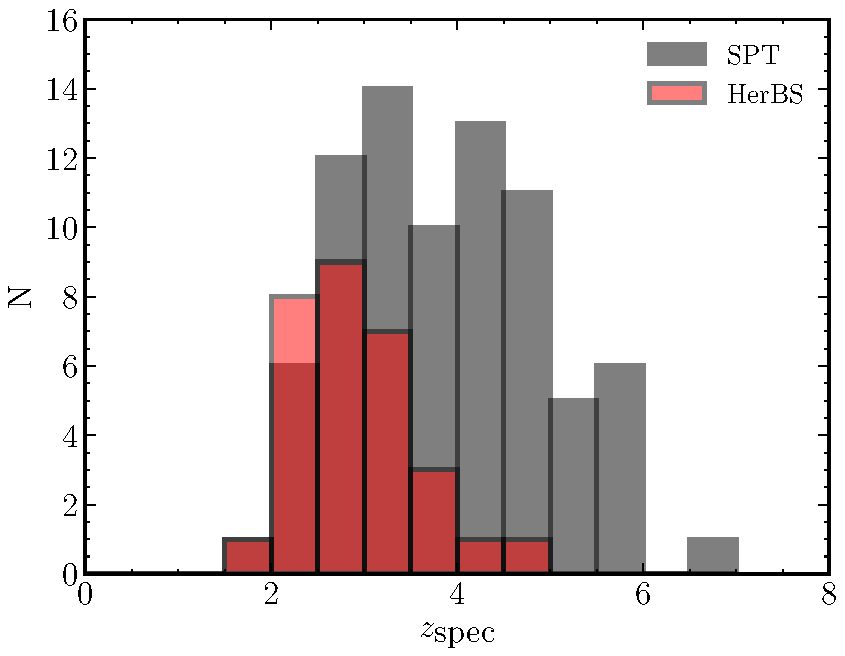
\includegraphics[width=0.5\columnwidth]{Figures/spt_herbs_redshift_distribution.pdf}
	\caption{The spectroscopic redshift distributions for the SPT-DSFG (grey) and HerBS (red) samples.}
	\label{fig:spt_herbs_redshift}
\end{figure}

\section{Far-Infrared and Sub-mm Colours}
\label{sec:fir_submm_colours}

A first estimate on the average dust properties of the two samples can be made by comparing their far-IR colours (which we define as the ratio between two flux densities in the FIR regime) with the predictions made using isothermal blackbody models. Previous studies have shown that FIR colours can be used as a proxy for dust properties (e.g. \citealt{Boselli_2010}; \citealt{Boselli_2012}; \citealt{Remy-Ruyer_2013}; \citealt{Smith_2019}) depending on the part of the FIR spectrum that the colour samples. For example, smaller wavelengths involving the \textit{Herschel}-PACS and \textit{Herschel}-SPIRE flux densities are more sensitive to changes in the dust temperature, while longer wavelengths are more sensitive to variations in the dust emissivity spectral index. In Figure \ref{fig:spt_herbs_colour_redshift} we show a selection of colours using flux densities between \textit{Herschel}-SPIRE 250\,\micron and ALMA 3\,mm that progressively travel across the spectrum from sampling the peak of thermal dust emission to the R-J tail. Using an isothermal modified blackbody model of the form $S_\nu \propto \frac{\nu^{\beta+3}}{e^{h \nu/kT} - 1}$, we predict the dependence of FIR colour on redshift for three combinations of dust temperature, $T_{\textrm{dust}}$, and $\beta$ ([T=30\,K, $\beta$=2], [T=30\,K, $\beta$=1.8] and [T=40\,K, $\beta$=2]). It can be seen that the assumed dust temperature has a significant effect on the location of the SED track for all FIR colours, while it is noticable that a change in $\beta$ has a larger effect on the observed colours at the longest wavelengths. 

Assuming for now that the dust emissivity index is well represented by $\beta \sim 2$ for all galaxies, then the FIR colours of most sources can be explained by a range of dust temperatures between T = 30 -- 40\,K assuming optically thin dust emission. There are notable exceptions, including a selection of SPT sources with high $S_{250\,\textrm{\micron}}/S_{500\,\textrm{\micron}}$ \todo[color=red]{Likely the 500um data, what does this imply?} and sources from both samples with high $S_{500\,\textrm{\micron}}/S_{3\,mm}$. At first this might suggest sources with large dust temperatures and/or high values of $\beta$, but other common culprits could be leading to these deviations from the bulk population. The most likely are the uncertainties on the flux density measurements or biases due to the choice of photometry. We note that our galaxies contain a combination of photometry obtained from single-dish observations (e.g. \textit{Herschel}, JCMT and SPT) and interferometers (ALMA). With their varying angular resolutions, emission observed with one instrument may be missed by another. In particular, we might expect that when ALMA resolves the single sources observed in the \textit{Herschel} wavebands into multiple components, some emission is lost giving the impression of higher FIR colours and thus higher dust temperatures and/or higher $\beta$.

In general, the SPT and HerBS galaxies occupy similar regions of the colour-redshift space, suggesting that the intrinsic dust properties of the two samples are likely to be similar. Given the scatter observed around the MBB models, it is appears unlikely that a single value of dust temperature and $\beta$ represents the observed SED of each galaxy equally well. \todo[color=red]{Description on how well the models represent the data - normalized distances should resemble a standardized normal distribution and colour-colour plots should be strongly correlated if the SEDs are well approximated by a single MBB with fixed beta.} 

The above results suggest that a single dust model assuming a constant $\beta$ value cannot explain the distribution of SEDs observed among the two populations. We are interested in ascertaining a single galaxy-integrated $\beta$, thus we must turn to fitting the observed SEDs individually to measure their dust properties. In the following we address two important questions about the properties of dust in high-redshift galaxies: i) is there diversity in the dust properties of high-redshift DSFGs? and ii) did these properties evolve over time? 


\begin{figure}
    \centering
    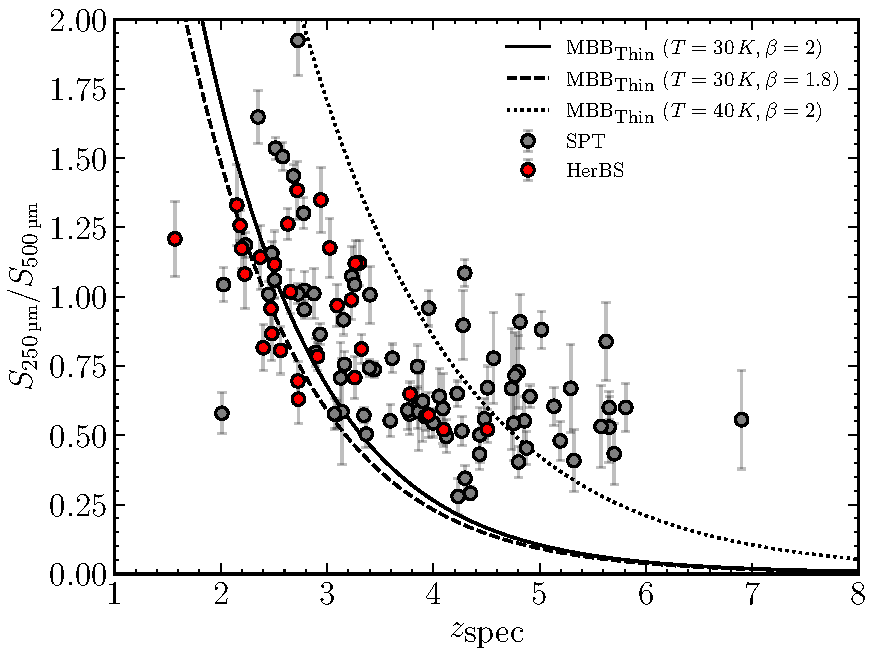
\includegraphics[width=0.5\columnwidth,height=0.26\textheight]{Figures/spt_herbs_colour_250_500.pdf}
    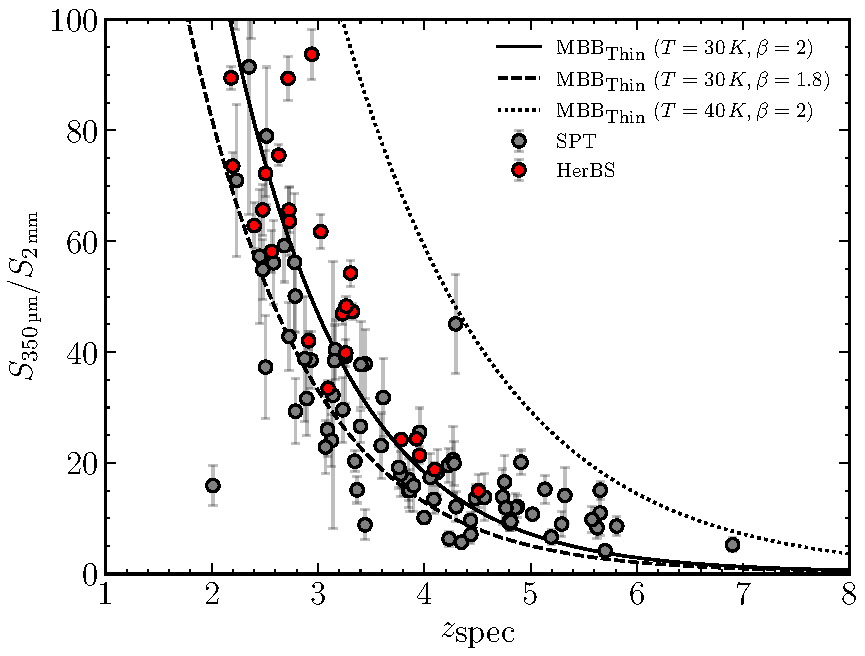
\includegraphics[width=0.5\columnwidth,height=0.26\textheight]{Figures/spt_herbs_colour_350_2000.pdf}
    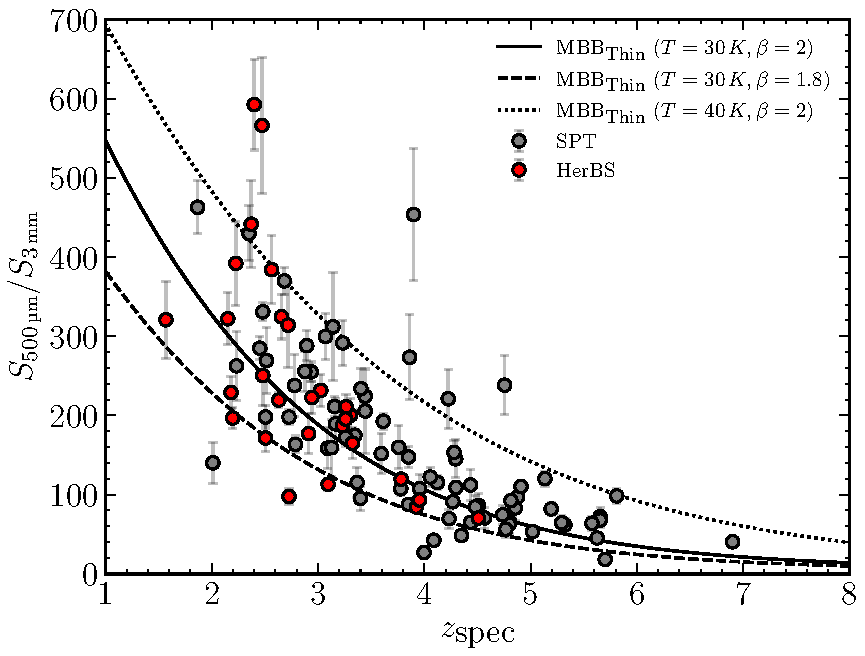
\includegraphics[width=0.5\columnwidth,height=0.26\textheight]{Figures/spt_herbs_colour_500_3000.pdf}
    \caption{Colour-redshift plots of X/X, X/X and X/X against spectrosopic redshift. The SPT sources are illustrated with grey circles and the HerBS sample as red circles. The predictions from three modified blackbody models assuming optical thin dust ([T = 30\,K, $\beta$=2], [T = 30\,K, $\beta$=1.8] and [T = 40\,K, $\beta$=2]) are plotted as solid, dashed and dotted black lines respectively.}
    \label{fig:spt_herbs_colour_redshift}
\end{figure}
\todo[color=orange]{Confirm which colours we am plotting here. They need only be progressively sampling longer wavelengths.}

\section{SED Fitting of DSFGs}

We modelled the FIR to millimeter spectra by fitting a single MBB model combined with a mid-IR power law to all sources. In the FIR to mm regime the SED is dominated by a modified Planck function that represents the cold dust reservoir from which most of the mass of dust in the ISM is contained. This "cold" dust resides in the diffuse ISM and is heated by the ambient interstellar radiation field. However, a lower fraction of dust by mass radiates at hotter temperatures, heated by nearby star-forming regions, young OB stars or AGNs which contributes substantially to a galaxy's IR luminosity and dominates the emission at rest frame wavelengths $\lesssim$ 70\,\micron. This mid-IR component can be approximated using a power law of dust temperatures of the form $S_\nu \propto \nu^{-\alpha}$, where a lower value of $\alpha$ represents a higher fraction of emission emananting from sources other than the cold reservoir of dust, and higher values asymptotically tending towards a modified blackbody, representing a single temperature of dust.

The modified blackbody form is a direct result of the radiative transfer equation, $\frac{dI_\nu}{ds} = -\kappa_\nu \rho I_\nu + j_\nu \rho$, where $\kappa_\nu$ represents the opacity of the dust, $\rho$ is the density, $j_\nu$ represents the emissivity of the dust and $I_\nu$ is the spectral radiance (per unit area). If we define the source function, $S_\nu$ as $j_\nu/\kappa_\nu$ and the frequency dependent optical depth as $d\tau_\nu = -\kappa_\nu \rho ds$, then the radiative transfer equation becomes $\frac{dI_\nu}{ds} = I_\nu - S_\nu = I_\nu - B_\nu$, where we have used the fact that at local thermal equilibrium (LTE) the source function is equal to the Planck function, $B_\nu(T)$. The solution to the radiative transfer equation takes the form $I_\nu = (1 - e^{-\tau_\nu}) B_\nu(T)$. Given that the spectral radiance is proportional to the flux density at a given frequency, we can rewrite this as the modified blackbody model:

\begin{equation}
	S_{\nu, \textrm{obs}} = \Omega(1 - e^{-\tau_\nu}) B_\nu(T_{\textrm{dust}}),
\label{eq:modified_blackbody_omega}
\end{equation}

where $\Omega$ represents the solid angle subtended by the galaxy. Assuming the comoving distance between the source and observer is $D$, then the source solid angle is given by the ratio between the projected area of the source on the sky and the square of the distance. Therefore,

\begin{equation}
	S_{\nu, \textrm{obs}} = \frac{\mu A}{D^2}(1 - e^{-\tau_\nu}) B_\nu(T_{\textrm{dust}}),
\label{eq:modified_blackbody_area}
\end{equation}

where $A$ is the area of the source and we have included a multiplicative factor $\mu$ to account for the possibility of magnification due to gravitational lensing. For any galaxy where there is no evidence to suggest that gravitational lensing is magnifying the source, we may set $\mu = 1$. The comoving distance is related to the luminosity distance, $D_L$, by the equation $D = D_L/(1+z)$, providing we assume a flat Universe where $\Omega_k = 0$ (\citealt{Hogg_1999}):

\begin{equation}
	S_{\nu, \textrm{obs}} = \frac{\mu A (1+z)}{D_L^2}(1 - e^{-\tau_\nu}) B_\nu(T_{\textrm{dust}}).
	\label{eq:modified_blackbody_area_dl}
\end{equation}

As suggested above, the optical depth, $\tau_\nu$, is defined as the product of surface mass density, $\Sigma_{\textrm{dust}} = M_{\textrm{dust}}/A$ and the dust opacity, $\kappa_\nu$, but is often assumed to take the form of a power law, $(\nu/\nu_1)^\beta$, where $\nu_1$ represents the frequency at which the optical depth equals unity, and thus the transition between optically thick and optically thin media. The dust opacity is also generally described by a power law, $\kappa_\nu = \kappa_0(\nu/\nu_0)^\beta$, where $\kappa_0$ is the emissivity of the grains per unit mass at some reference frequency $\nu_0$. Hereafter we shall adopt $\kappa_0 = 0.077$\,m$^2$kg$^{-1}$ at $\nu_0 = 353$\,GHz ($\lambda_0 = 850$\,\micron) \todo[color=green]{Add references}. Following substitution we find that

\begin{equation}
	S_{\nu, \textrm{obs}} = \frac{\mu A (1+z)}{D_L^2}\Bigg(1 - e^{- \frac{M_{\textrm{dust}}\kappa_\nu}{A}}\Bigg) B_\nu(T_{\textrm{dust}}).
	\label{eq:modified_blackbody_general_opacity_a}
\end{equation}

The final amendment to the MBB models is to account for the heating of the dust due to the ambient temperature of the Cosmic Microwave Background (CMB). At high redshifts the CMB becomes a non-negligible source of heating, which unaccounted for in the model, could bias estimates of the dust temperature and dust emissivity index. When the CMB temperature at the redshift of the galaxy is a significant fraction of the cold dust temperature of the ISM within the galaxy, then we observe a change in the shape of the FIR SED (\citealt{daCunha_2013}). At local thermal equilibrium, the increase in the ISM temperature due to CMB heating at higher redshifts ($T_{\textrm{CMB}} = T_{\textrm{CMB}, 0}(1+z)$, where $T_{\textrm{CMB}, 0}$ is the temperature of the CMB today = 2.72\,K) has two competing effects on the observed dust emission. First, the dust continuum emission is boosted by the increased temperature of the CMB; second, the increased temperature creates a stronger background from which we observe the dust continuum. The net result on the SED is explained further in \citealt{daCunha_2013}. We account for the effects of dust heating by the CMB using the procedure explained therein. The CMB-adjusted general opacity blackbody model is now given by 

\begin{equation}
	S_{\nu, \textrm{obs}} = f_{\textrm{CMB}}\frac{\mu A (1+z)}{D_L^2}\Bigg(1 - e^{- \frac{M_{\textrm{dust}}\kappa_\nu}{A}}\Bigg) B_\nu(T_{\textrm{dust}}(z)),
		\label{eq:modified_blackbody_general_opacity_a_cmb}
\end{equation}

where we have made two changes. First, the prefactor $f_{\textrm{CMB}}$ denotes the fraction of the total dust emission that is observed against the background of the CMB and is given by Equation 18 of \citealt{daCunha_2013}; $f_{\textrm{CMB}} = \frac{S_\nu^{\textrm{observed}}}{S_\nu^{\textrm{intrinsic}}} = 1 - \frac{B_\nu[T_{\textrm{CMB}}(z)]}{B_\nu[T_{\textrm{dust}}(z)]}$. Second, we have redefined the dust temperature to be a function of redshift, $T_{\textrm{dust}}(z)$, and is given by Equation 12 of \citealt{daCunha_2013}; $T_{\textrm{dust}}(z) = [T_{\textrm{dust}, 0}^{4+\beta} + T_{\textrm{CMB}, 0}^{4+\beta} ((1+z)^{4+\beta} - 1)]^{\frac{1}{4+\beta}}$, where $T_{\textrm{dust}, 0}$ is the dust temperature at a redshift of zero. Note that in all future references of the dust temperature of a galaxy, we refer to the luminosity-weighted, CMB-corrected temperature as defined above unless otherwise stated.

In this general form of the modified blackbody there are up to four parameters describing the dust properties of the galaxy: the dust mass, $M_{\textrm{dust}}$, the characteristic dust temperature, $T_{\textrm{dust}}$, the radial size of the source, $r$, and the dust spectral index, $\beta$. The simplest approximation one can make is that the dust emission is optically thin, $\tau_\nu \ll 1$, which simplifies the self opacity term from $(1 - e^{-\tau_\nu})$ to $\tau_\nu$, and removes the necessity for defining the size of the continuum emission:

\begin{equation}
	S_{\nu, \textrm{obs}} = f_{\textrm{CMB}}\frac{\mu (1+z)}{D_L^2}M_{\textrm{dust}}\kappa_\nu B_\nu(T_{\textrm{dust}}(z)).
	\label{eq:modified_blackbody_optically_thin}
\end{equation}

For completeness, the sources were modelled using the optically thin approximation (Equation \ref{eq:modified_blackbody_optically_thin}) and in the general scenario where dust is allowed to remain optically thick at FIR wavelengths (Equation \ref{eq:modified_blackbody_general_opacity_a}). Given how high the dust masses are expected to be for the \textit{Herschel} and SPT sources, it is not unreasonable to expect that the dust might be optically thick at wavelengths probed by our photometry (e.g. \citealt{Conley_2011}; \citealt{Casey_2019}; \citealt{Cortzen_2020}). 

Some of the SPT sources have intrinsic size measurements from lens modelling in \citealt{Spilker_2016}, although caution should be exercised when using such estimates as the size is measured at a particular wavelength (in this case at 870\,\micron with ALMA imaging), and it is unlikely to be the same at all wavelengths due to differential lensing. However, we assume no differential lensing and take the effective radii as the size of the dust continuum region for the [...]\todo[color=green]{Add number} SPT galaxies modelled in \citealt{Spilker_2016}. Their average size is $\sim$ 1\,kpc. The remaining SPT and HerBS sources without known sizes require an alternative way of constraining the dust opacity. From the definitions of the optical depth given above we see that the transitional frequency is given by $\nu_1 = \nu_0(\kappa_0 \Sigma_{\textrm{dust}})^\beta$. Common values of $\lambda_1$ are 100\,\micron and 200\,\micron (\citealt{Blain_2003}; \citealt{Draine_2006}; \citealt{Conley_2011}; \citealt{Rangwala_2011}; \citealt{Greve_2012}; \citealt{Casey_2014}; \citealt{Spilker_2016}; \citealt{Casey_2019}; \citealt{Cooper_2022}; \citealt{Drew_2022}). For comparison with other works in the literature, we made no prior assumption about the value of $\lambda_1$ and modelled the SEDs of all sources assuming a value of 100\,\micron and 200\,\micron. In Section \ref{sec:comparison_optically_thin_and_general_opacity} we evaluate which approximation is most suitable by comparing the derived parameters for the SPT sources with lens models and with well studied sources in the literature that have had their dust opacities measured.

The lensing magnifications required to calculate the instrinsic properties of the sources come from the lens modelling in \citealt{Spilker_2016} for the SPT-DSFGs and from \citealt{Urquhart_2022} for the HerBS sample. The SPT-DSFGs range in magnification factors from 1 to 33, with a median value $\mu_{\textrm{median}} = 5.5$ which is assumed for all SPT sources not included in the study of \citealt{Spilker_2016}. The magnification factors of HerBS sources are derived in a different manner. It is well known that there is a correlation between the CO luminosities of submillimeter galaxies and their line widths (\citealt{Bothwell_2013}; \citealt{Dannerbauer_2017}; \citealt{Neri_2020}), in a CO analogy of the Tully-Fisher relationship (\citealt{Tully_1977}). The effect of gravitational lensing is to amplify the apparent CO luminosity, while the line width is unaffected. The offset from the relationship defined by a population of unlensed sources can then be used to estimate the extent to which a source is being lensed. In the case of the HerBS sources in this study, the magnification factors are in the range 1 -- 50 and the median is $\mu_{\textrm{median}}$ = 5.3.

During SED fitting we assumed flat priors on the dust mass between $10^5$ -- $10^9\,M_\odot$, the dust temperature between $T_{\textrm{CMB}}$ -- 100\,K, $\beta$ between 0.5 -- 6 and $\alpha$ between 0.5 -- 8. If a measurement of the intrinsic size of the source is available it is used during fitting, otherwise we assumed $\lambda_1$ = 100\,\micron and $\lambda_1$ = 200\,\micron in two separate applications of the general opacity model. The best fitting SEDs are determined from a Markov Chain Monte Carlo (MCMC) algorithm using the \texttt{emcee} package (\citealt{Foreman-Mackey_2013}) and assuming the general opacity model of Equation \ref{eq:modified_blackbody_general_opacity_a_cmb} and the optically thin model of Equation \ref{eq:modified_blackbody_optically_thin}. The dust properties are taken to be the median of their respective posterior distributions with 1$\sigma$ uncertainties quoted at the 16th and 84th percentiles. 

Calibration errors are added in quadrature with the flux density uncertainties during the fitting process according to an additional 7\% (\textit{Herschel}-PACS), 5.5\% (\textit{Herschel}-SPIRE), 5\% (SCUBA-2), 12\% (APEX-LABOCA), 7\% (SPT) and 10\% (ALMA). For consistency across the literature, we have conformed to the "best practices" outlined in \citealt{Drew_2022}. These recommendations aim to make cross-referencing comparisons between studies easier and provide a set of guidelines that allows the community to compare the dust properties of different galaxy populations coherently. In brief, these guidelines are: 

\begin{enumerate}
	\item Galaxies that lack photometric coverage should not be fit with models containing more free parameters than data. In the case of the MBB models used here, the maximum number of free parameters are five for the general opacity model ($M_{\textrm{dust}}$, $T_{\textrm{dust}}$, $\beta$, $\alpha$ and $r$/$\lambda_1$) and four when using the optically thin approximation ($M_{\textrm{dust}}$, $T_{\textrm{dust}}$, $\beta$ and $\alpha$), whereas there are no sources with fewer than six photometric constraints in the SPT-DSFG sample, and no sources with fewer than five in the HerBS sample.
	\item The number of free parameters should vary depending on the available photometric constraints. It is also recommended that Gaussian priors be used where data have low SNR and the parameters be fixed where data is limited, especially for $\lambda_1$ if there are no independent measurements for the dust column density. In this study we assume flat priors on all parameters given that we do not know the prior distribution and this will not be inferred through Hierarchical Bayesian fitting (see \citealt{Lamperti_2019} for an example of this method). However, in accordance with the best practices, we fix the wavelength where the dust opacity reaches unity either directly or indirectly from the galaxy's intrinsic size, given that we do not have substantial enough photometric coverage to constrain this parameter well.
	\item Poorly sampled SEDs that have no spatially-resolved dust continuum observations should focus on constraining the rest-frame peak wavelength $\lambda_{\textrm{peak}}$ rather than the dust temperature. As will be mentioned later, we do not consider the characteristic dust temperature obtained from our fits to be the true temperature of the dust, but rather a single, luminosity-weighted value that describes the bulk of the dust by mass in the ISM. Later we shall define an alternative dust temperature for the \textit{Herschel} and SPT galaxies as defined by their peak wavelength which is less biased by the choice of SED model.
\end{enumerate}

\section{Results of SED Fitting}

\subsection{Example SEDs: HerBS-11 and SPT0002-52}

In Figure \ref{fig:example_SEDs} we show the SED modelling of the first source alphanumerically in the two samples, HerBS-11 and SPT0002-52. Both sources do not have measurements for their intrinsic size and so two general opacity models are assumed, $\lambda_1$ = 100\,\micron and 200\,\micron. The SEDs of all other sources can be found in Appendices \ref{app:HerBS_SEDs} and \ref{app:SPT_DSFG_SEDs}. Our first look at how well the dust properties are constrained is to study the posterior distributions obtained from the converged MCMC chains of HerBS-11 and SPT0002-52. In the bottom panels of Figure \ref{fig:example_SEDs} we show the joint posterior distributions for the two sources. As was predicted from the FIR/sub-mm colours presented in Section \ref{sec:fir_submm_colours}, the two sources have similar posterior distributions that probe similar ranges in the parameter space. The most notable difference is that the parameter $\alpha$ is not constrained with any model for HerBS-11, which can be seen in the spread of acceptable SEDs as a result of having no \textit{Herschel}-PACS photometry. We note, however, that this has little effect on the dust properties of the cold ISM and is better than fitting an isothermal model to all datapoints which would skew the results to much higher average temperatures. 

Common to both sources is the offset in some parameters depending on the opacity model that is being used. The optical depth and the dust temperature are strongly correlated such that an increase in the dust temperature and a decrease in the optical depth both shift the peak of the SED to shorter wavelengths. Then, given the relationship between the dust mass and dust temperature, \todo[color=orange]{provide relationship} the deviations of the optical depth from the truth leads to systematic offsets in the derived dust temperatures and dust masses. These systematics can be troubling for studies at high redshift where there is already tension about the mass of the ISM in dust and the modelling required to predict the ISM growth at such early epochs, otherwise known as the dust budget crisis (e.g. \citealt{Rowlands_2014}). On the other hand, some parameters appear to be well constrained and relatively indifferent to dust opacity. For example, the dust emissivity spectral indices show reasonable agreement given it is defined by the slope of the R-J tail which is relatively insensitive to the dust opacity and constrained by photometry which may lie comfortably within the optically thin approximation. To circumvent most of the uncertainty in the dust temperature ascribed to the choice of model, we preferentially adopted $\lambda_\textrm{peak}$ as a proxy for the average dust temperature of the dust, as this value is a fundamental property of the SED that is minimally affected by model assumptions. Note that while opacity assumptions are required to translate $\lambda_\textrm{peak}$ into a dust temperature, the peak wavelength itself may be used for comparisons between studies. Similarly, the IR luminosity, derived by integrating the dust SED between 8\,\micron and 1000\,\micron, is a fundamental quantity that is defined by the shape of the SED and thus not largely affected by our model assumptions. It is for these reasons that previous studies have used the integrated bolometric luminosity and the peak wavelength of galaxies' dust emission to assess whether dust temperatures and the DSFG contribution to the IR galaxy luminosity function (IRLF) evolved with redshift (e.g. \citealt{Casey_2018}; \citealt{Drew_2022}).


\begin{figure}
	\centering
	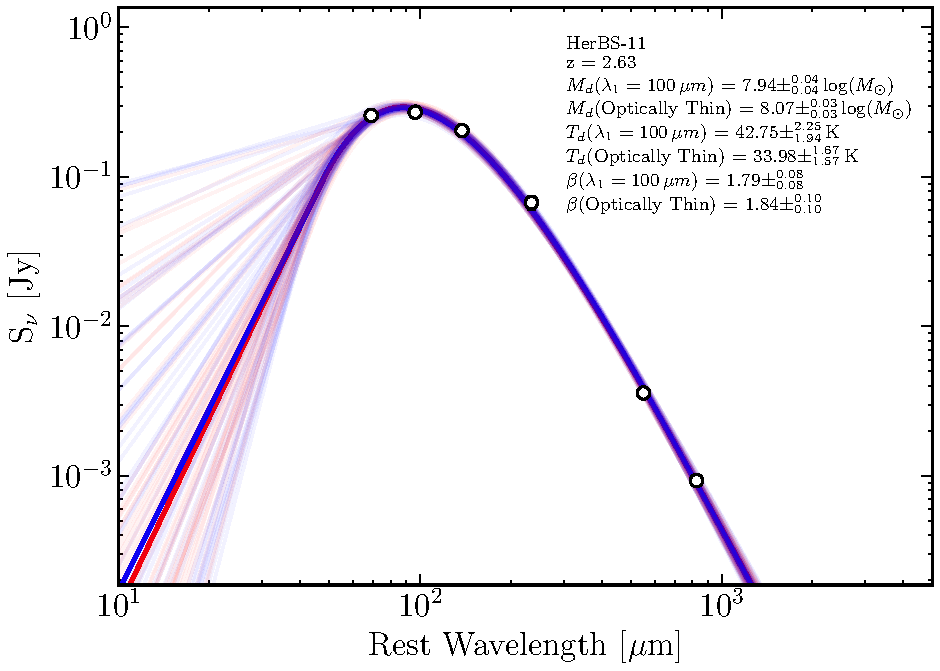
\includegraphics[width=0.49\columnwidth]{Figures/herbs_sed_example.pdf}
	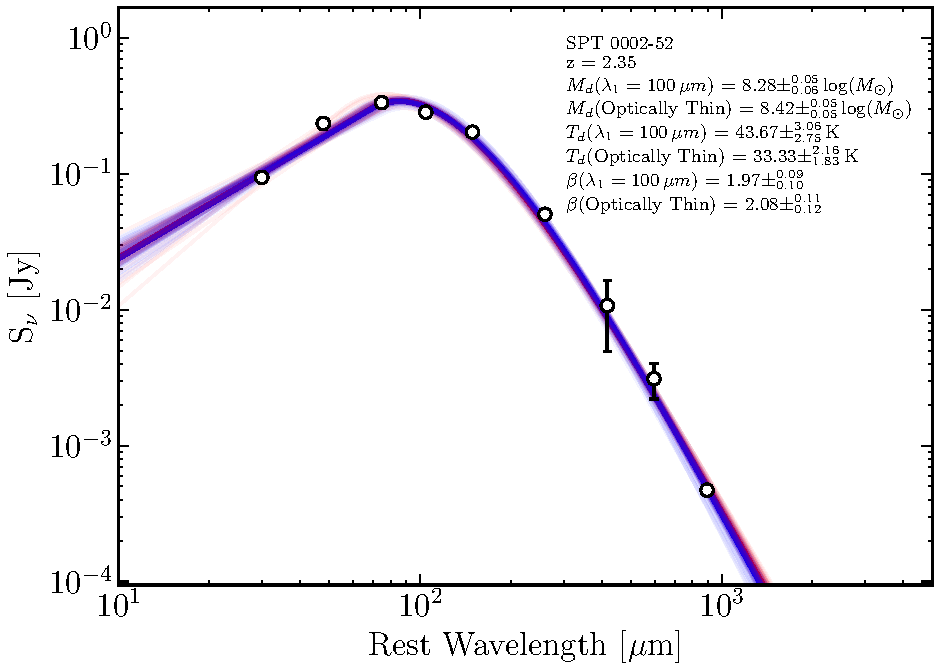
\includegraphics[width=0.49\columnwidth]{Figures/spt_sed_example.pdf}
	\includegraphics[width=0.49\columnwidth]{Figures/herbs_example_contours.pdf}
	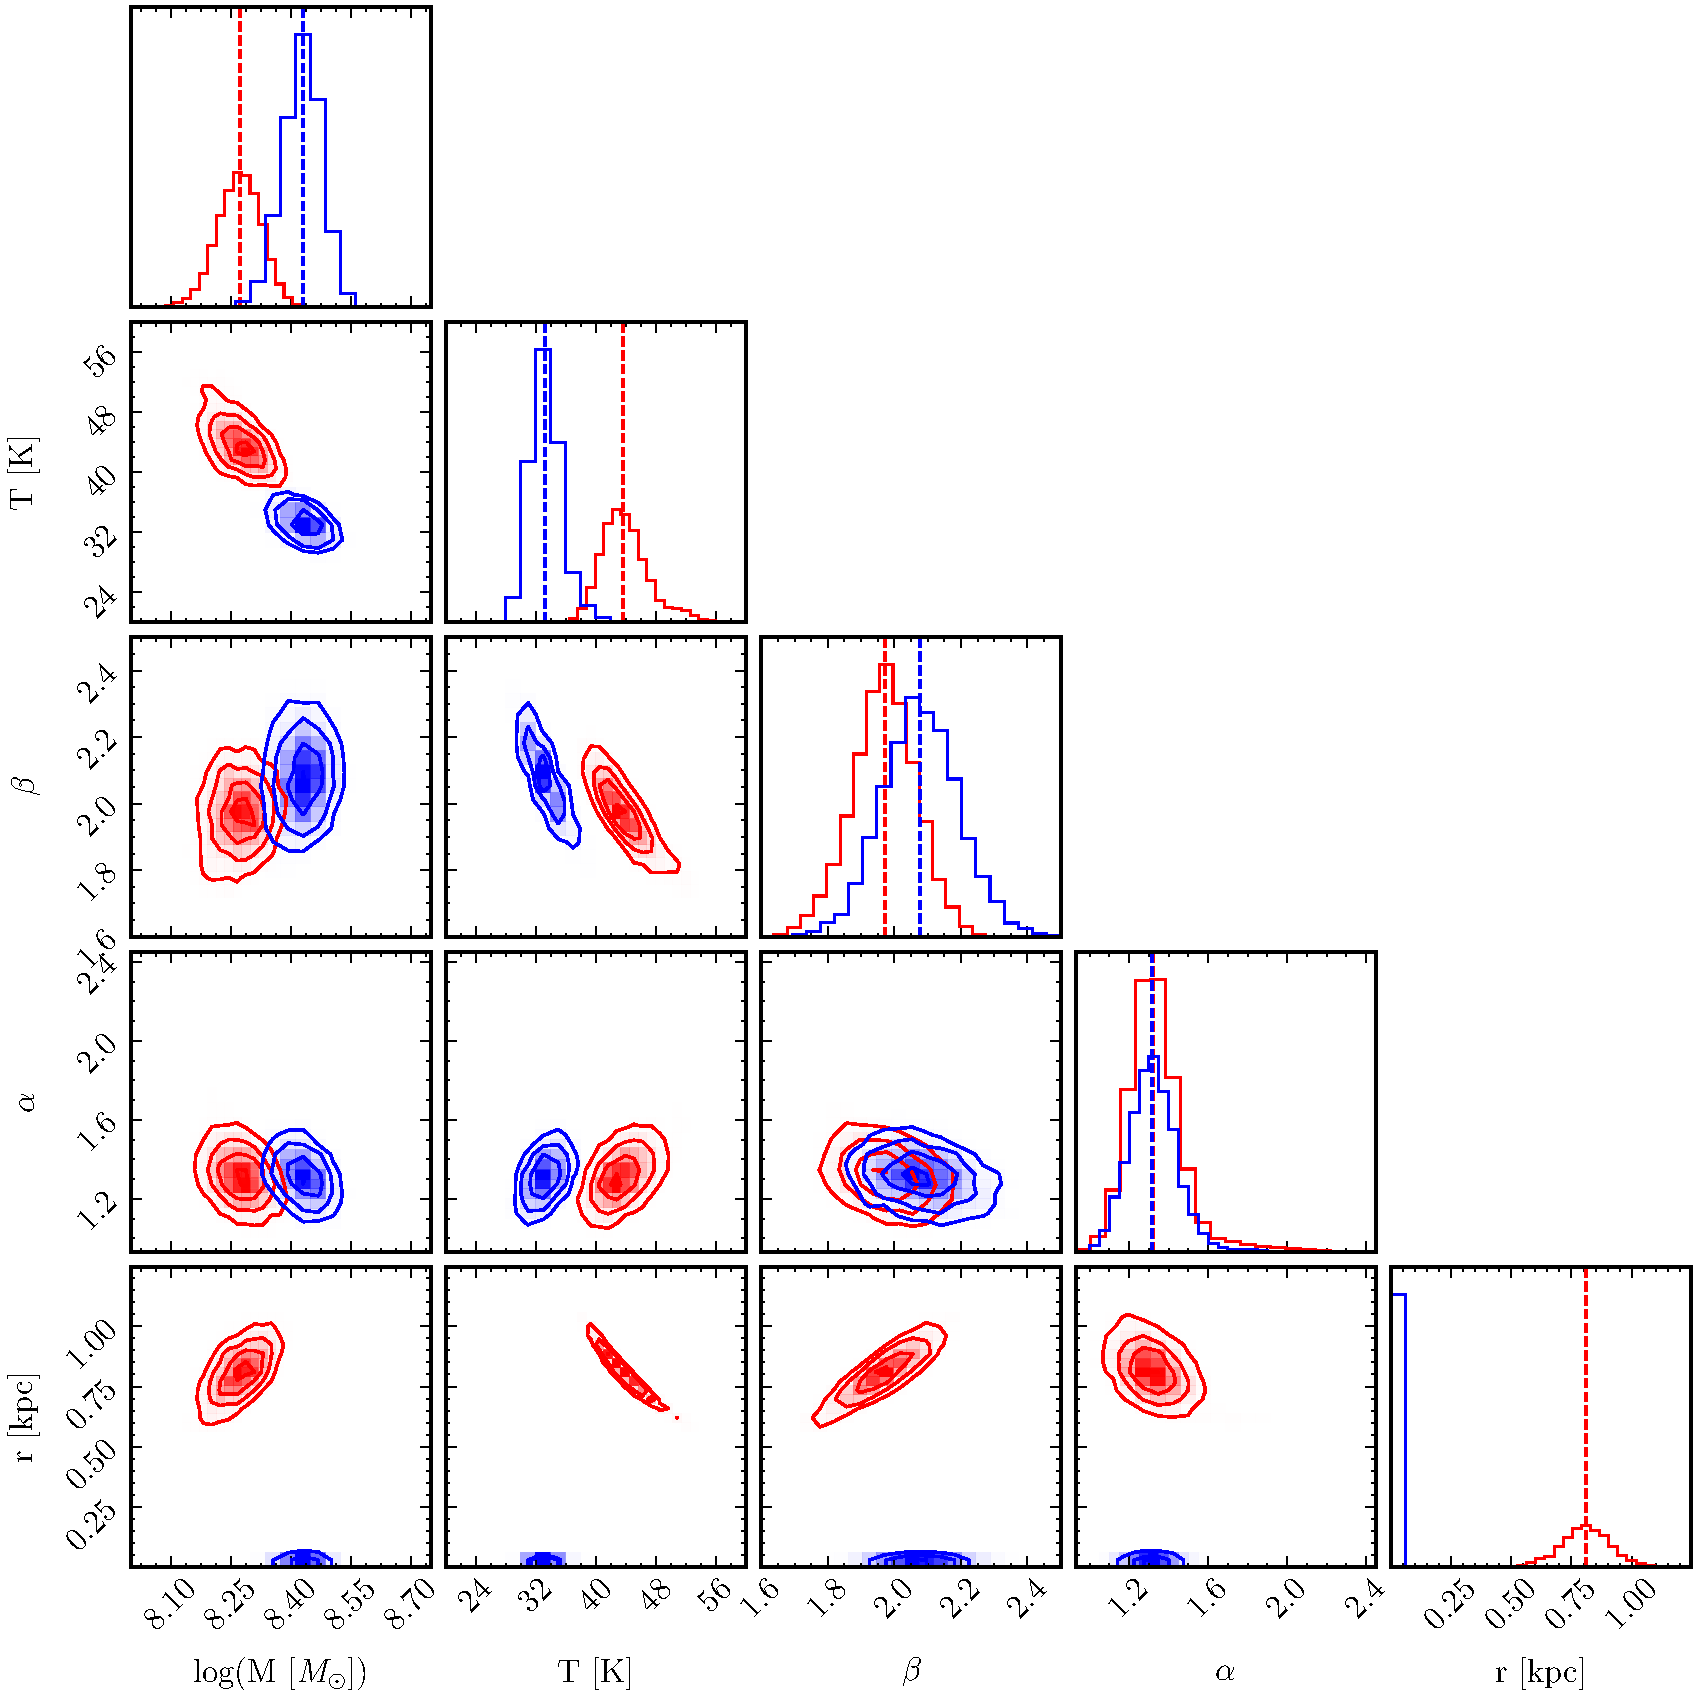
\includegraphics[width=0.49\columnwidth]{Figures/spt_example_contours.pdf}
	\caption{Top: Example SED fits for HerBS-11 and SPT002-52. The best fitting optically thin and general opacity models, taken as the median value for each fitting parameter, are illustrated as thick red (optically thin), blue ($\lambda_1$ = 100\,\micron) and green ($\lambda_1$ = 200\,\micron) lines. The range of accepted SED fits are shown from 500 random draws from the posterior distribution, illustrated as the shaded regions following the same colour convention. Bottom: The joint posterior distributions of HerBS-11 and SPT0002-52. The fitting parameters illustrated are the dust mass, the dust temperature, $\beta$ and $\alpha$. The derived parameters, IR luminosity and the peak wavelength, are also included.}
	\label{fig:example_SEDs}
\end{figure}

[*** This is where I am up to in editing ***]

\subsection{Comparison between Optically Thin Approximation and General Opacity Models}
\label{sec:comparison_optically_thin_and_general_opacity}

The distribution of the dust properties is shown by the stacked posterior distributions for all sources in Figure \ref{fig:stacked_posteriors}. Relevant parameters are shown with the lensing magnification included as this more closely resembles the set of observables. By not including the magnification factor we find a wider and less smooth posterior distribution for dust masses and IR luminosities. The median values of each parameter, averaged over the SPT and HerBS samples, were taken to be the median of the stacked posterior distribution with errors again quoted at the 16th and 84th percentiles. A summary of the average values for each parameter is given in Table \ref{tab:parameter_results}. The main parameter of interest, the dust emissivity speactral index, is well constrained at values of approximately 1.8 -- 2, which is in good agreement with the commonly accepted values for Galactic dust and nearby galaxies. Further discussion on this apparent lack of redshift evolution in $\beta$ is given in Section. \todo[color=green]{Add reference when written} The small increase in the average $\beta$ for SPT galaxies is likely a result of the lower average dust temperature given the strong degeneracy between the two parameters, and as mentioned earlier, this offset in dust temperature is likely due to our opacity assumptions. We note, however, that all parameters derived from the optically thin approximation are in agreement with their general opacity counterparts to within 1$\sigma$. This would suggest that, providing suitable constraints are made on the optical depth (ideally with a priori knowledge or informed from the literature) then either model is equally sufficient at describing the SEDs of high redshift galaxies, especially if $\lambda_{\textrm{peak}}$ is used as a proxy for the dust temperature in subsequent analysis. 

\begin{table}
    \centering
    \begin{tabular}{|p{3cm}|p{3cm}|p{3cm}|p{3cm}|p{3cm}|}
        \hline
        Parameter & HerBS & SPT & HerBS & SPT \\ 
		& General Opacity & General Opacity & Optically Thin & Optically Thin \\
        \hline
        \hline
        log($\mu M_{\textrm{dust} [M_\odot]}$) & $9.08_{-0.21}^{+0.14}$ & $9.07_{-0.38}^{+0.48}$ & $9.11_{-0.15}^{+0.22}$ & $9.21_{-0.35}^{+0.42}$ \\
		$T_{\textrm{dust}}$ [K] & $42.95_{-8.43}^{+4.64}$ & $37.23_{-7.55}^{+7.99}$ & $34.37_{-6.66}^{+4.14}$ & $30.32_{-6.71}^{+8.25}$ \\
		$\beta$  & $1.76_{-0.21}^{+0.24}$ & $1.92_{-0.38}^{+0.40}$ & $1.83_{-0.26}^{+0.34}$ & $2.00_{-0.43}^{+0.50}$ \\
		log($\mu L_{\textrm{IR} [L_\odot]}$) & $13.66_{-0.24}^{+0.21}$ & $13.96_{-0.31}^{+0.21}$ & $13.65_{-0.36}^{+0.20}$ & $13.94_{-0.32}^{+0.21}$ \\
		$\lambda_{\textrm{peak}}$ [$\mu$m] & $88.38_{-5.76}^{+13.10}$ & $93.60_{-11.72}^{+15.55}$ & $88.13_{-6.39}^{+12.72}$ & $93.69_{-11.79}^{+14.62}$ \\
        \hline
    \end{tabular}
    \caption{Caption.}
    \label{tab:parameter_results}
\end{table}

[Compare with literature values of $\lambda_1$ from Witstok+2023]

While we have illustrated that the differences between the general opacity and optically thin models are small and systematic, it is not yet clear that the results obtained using the approximation $\lambda_1$ = 100\,\micron, which is used for many of the SPT galaxies and all HerBS galaxies, is in keeping with the sources where we had greater knowledge of the dust opacity from their intrinsic size. In the lower panel of Figure \ref{fig:stacked_posteriors} we show the SPT stacked posterior distributions for each parameter in the general opacity model split according to the subset of those which were derived assuming a fixed value of $r$ and those derived assuming $\lambda_1$ = 100\,\micron. We see that assuming a fixed value for $\lambda_1$ informed a priori leads to derived dust properties similar to those where the dust continuum area is known. The notable differences are a possible extended tail to higher dust temperatures and an offset to lower IR luminosities for the $\lambda_1$-derived subset. The agreement between the two subsamples would suggest that our approximation is valid. As we do not have radial sizes of any HerBS galaxies, we can not make the same comparison and rely on the fact that the samples occupy similar regions of parameter space to validate the use of $\lambda_1$ = 100\,\micron.

\todo[color=orange]{Show 200-micron fits?}

\begin{figure}
	\centering
	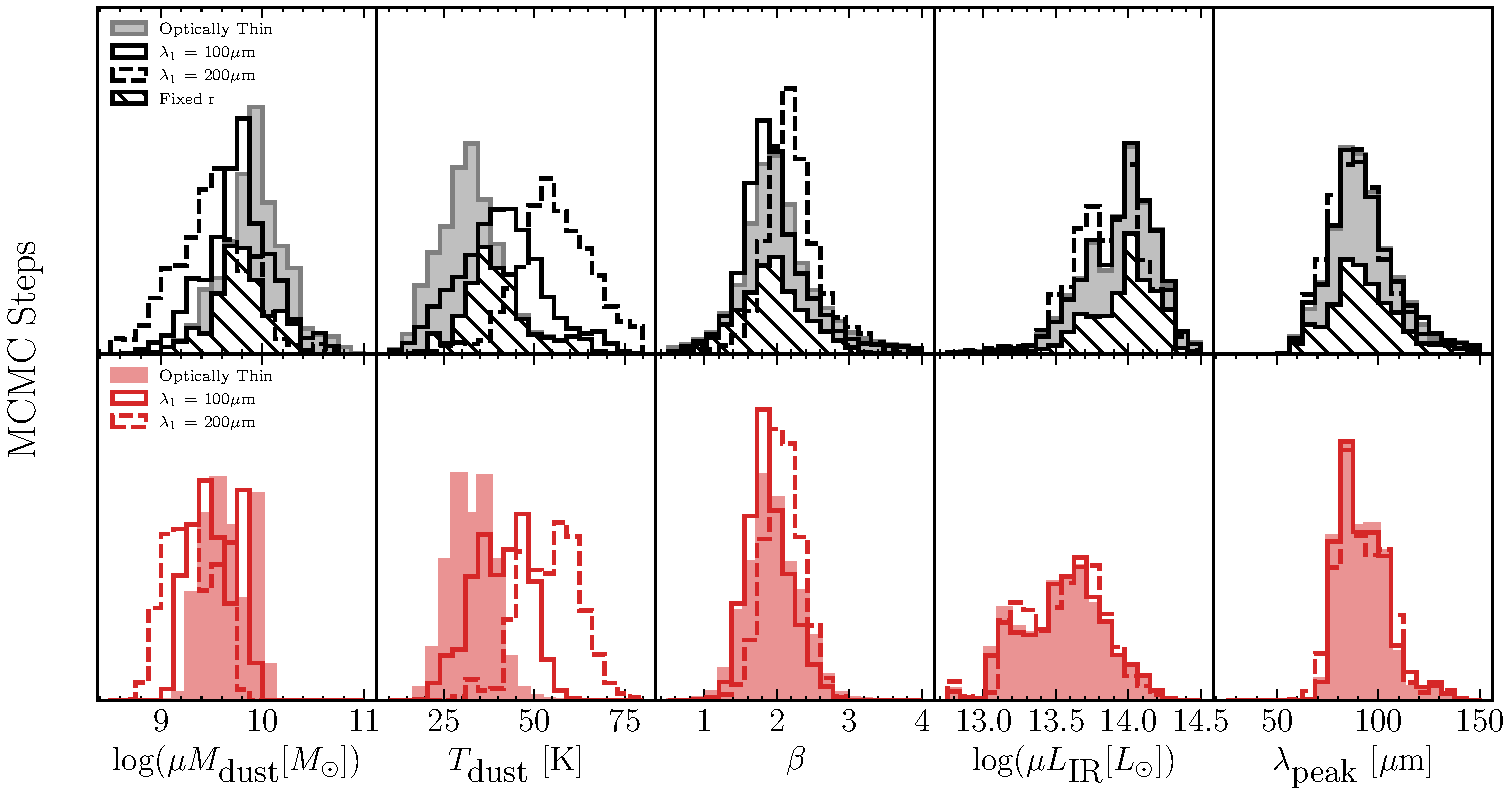
\includegraphics[width=\columnwidth]{Figures/stacked_posterior.pdf}
	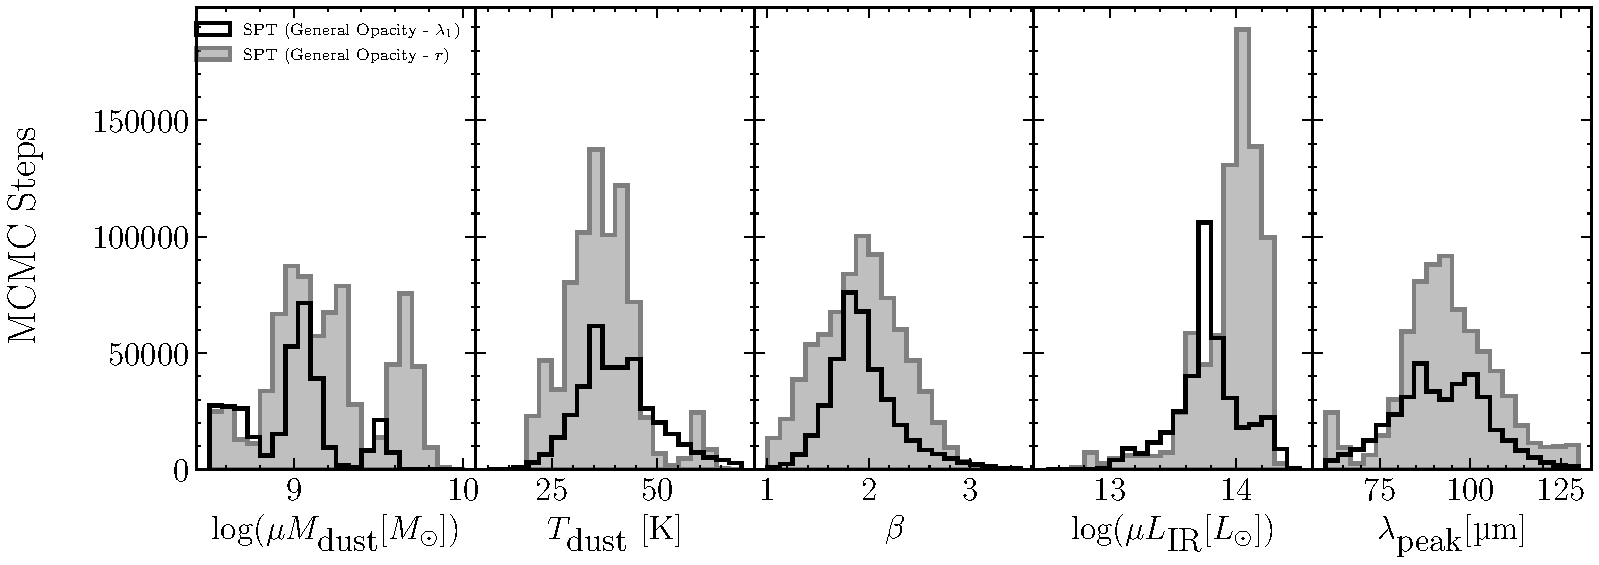
\includegraphics[width=\columnwidth]{Figures/stacked_posterior_SPT.pdf}
	\caption{Caption.}
	\label{fig:stacked_posteriors}
\end{figure}

The optically thin, isothermal MBB model is widely used in the literature (\citealt{Magdis_2012}; \citealt{Dudzeviciute_2020}; \citealt{daCunha_2021})

[Note quantitatively the difference in parameter values as a way to "imaginary-correct" as needed]

[To ensure our results are not biased by badly fit SEDs, we have reduced the analysis hereafter to include only sources where the reduced chi squared of the fit is less than two, leaving 12 HerBS and 30 SPT galaxies that have suitable fits regardless of the opacity assumptions. Note that there are only a handful of sources where the choice of model moves the galaxy from inclusion to exclusion based on the reduced chi-square value and thus their omission would not alter our conclusions.]

[Why we choose to continue on the optically thin approximation -> beta is almost certainly indifferent from R-J tail -> we can resolve T problems by using peak wavelength.]


\subsection{The $\beta$-Dust Temperature Degeneracy}

[Correlations in parameters -> show posteriors and individual values together -> Beta-T correlation -> we will use simulations to see if this is a real effect]

There is a known degeneracy between the dust temperature and $\beta$, which has been observed in a wide variety of scenarios in which the isothermal MBB has been used, from clouds in the Galaxy to galaxy-integrated $\beta$-T relationships from IR luminous galaxies (\citealt{Dupac_2003}; \citealt{Desert_2008}; \citealt{Paradis_2010}; \citealt{Schnee_2010}; \citealt{Veneziani_2010}; \citealt{Bracco_2011}; \citealt{Galametz_2012}; \citealt{Paladini_2012}; \citealt{Smith_2012}; \citealt{Lamperti_2019}; \citealt{daCunha_2021}).

[*** End of editing ***]

\section{Simulations}

In order to assess how accurately our fitting routine derives a galaxy's dust parameters, we ran a suite of mock SEDs with known input parameters and measured how precisely we recover the dust properties from our fits. There are three main aims of running input-output simulations of our SPT and HerBS galaxies: i) it provides a quantitative error on our dust parameters, beyond those estimated from their respective posterior distributions, that tell us the scatter we might expect our dust properties to have from their true value; ii) we can test whether our main parameter of interest, $\beta$, is susceptible to variation due to the degeneracy with dust temperature. By providing a hypercube of parameters, any correlations observed in the output parameters can be attributed to the fitting process, which would otherwise be mistakenly taken as a physical correlation when applied to real galaxies; iii) the photometric bands sample the SEDs at the same observed wavelengths, corresponding to different rest frame wavelengths at different redshifts. The variation in sampling of the rest-frame SED with redshift could introduce biases in the measured dust properties, which would hinder our conclusions about the evolution of the average dust properties of DSFGs with redshift.

We generated the mock SEDs in the following way. First we must assume that the dust emission can be described by an isothermal blackbody in the optically thin regime (Equation \ref{eq:modified_blackbody_optically_thin}). A catalogue of {\color{red} X} models are produced with random parameters uniformly distributed between the lower and upper bounds presented in Table \ref{tab:simulation_inputs}, which are chosen to reflect the width of the posterior distributions observed for the real sources. To recreate mock galaxies with SEDs that reflect the properties of the HerBS and SPT samples the simulations were run twice. In the first instance each mock SED was placed at a random redshift between {\color{red} X} and {\color{red} X} and evaluated at the observed wavelengths of the HerBS sources. Note, however, that we did not include observations at 1.2\,mm as few sources in the final sample have photometric constraints at this wavelength, but all other wavelengths are included which results in a best scenario situation. Given the completeness of the \textit{Herschel} observations at all three SPIRE wavelengths and our requirement of having at least two constraints on the R-J tail at $\lambda_{\textrm{obs}}$ > 1\,mm, the inclusion of all wavelengths is a good approximation of our final HerBS sample. In a similar manner, in the second simulation, each iteration of input parameters is distributed between redshifts {\color{red} X} and {\color{red} X}, reflecting the wider SPT redshift distribution, and the flux density measured at each observed wavelength of the SPT sample. Using the flux density errors for each source in the final sample, the range of SNR values was used to define a random error on each flux. Each flux density was then perturbed by a value generated from a normal distribution with a width equal to the mock galaxy's flux density error at that wavelength to represent the typical observational errors.

\begin{table}
    \centering
    \begin{tabular}{|p{3cm}|p{3cm}|p{3cm}|p{3cm}|p{3cm}|}
        \hline
        Parameter & Bounds \\
        \hline
        \hline
        log($\mu M_{\textrm{dust} [M_\odot]}$) & \\
		$T_{\textrm{dust}}$ [K] &  \\
		$\beta$  &  \\
		$\alpha$  &  \\
        \hline
    \end{tabular}
    \caption{Caption.}
    \label{tab:simulation_inputs}
\end{table}

Each simulated galaxy carried with it a flag corresponding to whether it would have been included in their respective sample, having been perturbed by observational error. A source is deemed not detected if any of the perturbed flux densities falls below 29\,mJy at 250\,\micron or 80\,mJy at 500\,\micron for the HerBS simulation or below 25\,mJy at 870\,\micron or 10\,mJy at 1.4\,mm for the SPT simulation.

\section{Possible Redshift Evolution in Dust Properties}

\section{Conclusions}

\listoftodos